\documentclass[12pt, twoside]{article}
\input{../preamble}

\fancyhead[LO]{La Scuola d'Italia / Dr.\ Huson / IB Math: Probability \\* 13 March 2026}
\fancyhead[RO]{Markscheme}
\fancyfoot[C]{\thepage}

\begin{document}
\subsubsection*{4.19 Quiz: Probability Review --- Markscheme}

\begin{enumerate}[itemsep=0.1cm]

%--- Problem 1: Venn diagram reading [7 marks] ---
\item In a class of 32 students, some do Music ($M$) and some do Drama ($D$).

\begin{center}
\vspace{-0.3cm}
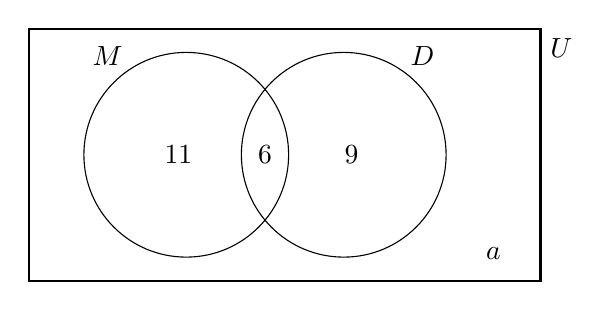
\begin{tikzpicture}
  \draw[thick] (0,0) rectangle (6.5,3.2);
  \node[anchor=north west] at (6.5,3.2) {$U$};
  \draw (2.0,1.6) circle (1.3cm);
  \node at (1.0,2.85) {$M$};
  \draw (4.0,1.6) circle (1.3cm);
  \node at (5.0,2.85) {$D$};
  \node at (1.9,1.6) {$11$};
  \node at (3.0,1.6) {$6$};
  \node at (4.1,1.6) {$9$};
  \node at (5.9,0.35) {$a$};
\end{tikzpicture}
\vspace{-0.3cm}
\end{center}

\begin{enumerate}[itemsep=0.3cm]
  \item Write down the number of students who do Music. \hfill [1]

  $n(M) = 11 + 6 = 17$ \hfill \textbf{(A1)}

  \item Find the number of students who do neither Music nor Drama, $a$. \hfill [1]

  $a = 32 - 11 - 6 - 9 = 6$ \hfill \textbf{(A1)}

  \item One student is chosen at random. Find the probability that
  \begin{enumerate}[label=(\roman*), itemsep=0.3cm]
    \item the student does not do Music; \hfill [1]

    $\mathrm{P}(M') = \dfrac{9 + 6}{32} = \dfrac{15}{32}$ \hfill \textbf{(A1)}

    \item the student does Music or Drama, but not both. \hfill [2]

    Identifying the correct regions: $11 + 9 = 20$ \hfill \textbf{(M1)}

    $\mathrm{P} = \dfrac{20}{32} = \dfrac{5}{8}$ \hfill \textbf{(A1)}
  \end{enumerate}

  \item Given that a student does Drama, find the probability that they also do Music. \hfill [2]

  Recognizing conditional probability, $n(D) = 6 + 9 = 15$ \hfill \textbf{(M1)}

  $\mathrm{P}(M \mid D) = \dfrac{6}{15} = \dfrac{2}{5}$ \hfill \textbf{(A1)}
\end{enumerate}

\newpage

%--- Problem 2: Two-way table + independence [6 marks] ---
\item The following table shows whether 16 students are in the IB math program
and whether they have a TI nSpire calculator.

\renewcommand{\arraystretch}{1.4}
\begin{center}
\begin{tabular}{|r|c|c|c|}
    \hline
    & nSpire & No nSpire & Total \\
    \hline
    IB        & 8  & 2  & 10 \\
    \hline
    Non-IB    & 1  & 5  & 6 \\
    \hline
    Total     & 9  & 7  & 16 \\
    \hline
\end{tabular}
\end{center}

\begin{enumerate}[itemsep=0.3cm]
  \item Find the probability that a randomly chosen student is in IB
        and has a nSpire. \hfill [1]

  $\mathrm{P}(\text{IB} \cap \text{nSpire}) = \dfrac{8}{16} = \dfrac{1}{2}$ \hfill \textbf{(A1)}

  \item Find $\mathrm{P}(\text{nSpire} \mid \text{non-IB})$. \hfill [2]

  Identifying non-IB total: $n(\text{non-IB}) = 6$ \hfill \textbf{(M1)}

  $\mathrm{P}(\text{nSpire} \mid \text{non-IB}) = \dfrac{1}{6}$ \hfill \textbf{(A1)}

  \item Determine whether ``is in IB'' and ``has a nSpire'' are
        independent events.
        Show your working and justify your answer. \hfill [3]

  $\mathrm{P}(\text{IB}) \times \mathrm{P}(\text{nSpire})
    = \dfrac{10}{16} \times \dfrac{9}{16}
    = \dfrac{90}{256} \approx 0.352$ \hfill \textbf{(M1A1)}

  $\mathrm{P}(\text{IB} \cap \text{nSpire}) = \dfrac{8}{16} = 0.5$

  $0.352 \neq 0.5$, so the events are \textbf{not independent}. \hfill \textbf{(R1)}
\end{enumerate}

\newpage

%--- Problem 3: Tree diagram [7 marks] ---
\item At a school, 60\% of students take the bus and 40\% walk.
Of those who take the bus, 10\% arrive late.
Of those who walk, 5\% arrive late.

\begin{enumerate}[itemsep=0.3cm]
  \item Complete the tree diagram below, showing all probabilities. \hfill [2]

  Missing values: Walk $= 0.4$; Bus on time $= 0.90$;
  Walk late $= 0.05$; Walk on time $= 0.95$ \hfill \textbf{(A1A1)}

  Compound probabilities:

  \begin{tabular}{ll}
    Bus $\cap$ Late: $0.6 \times 0.10 = 0.06$ &
    Bus $\cap$ On time: $0.6 \times 0.90 = 0.54$ \\
    Walk $\cap$ Late: $0.4 \times 0.05 = 0.02$ &
    Walk $\cap$ On time: $0.4 \times 0.95 = 0.38$ \\
  \end{tabular}

  \item Find the probability that a randomly chosen student walks and
        arrives late. \hfill [1]

  $\mathrm{P}(\text{Walk} \cap \text{Late}) = 0.4 \times 0.05 = 0.02$ \hfill \textbf{(A1)}

  \item Find the probability that a randomly chosen student arrives late. \hfill [2]

  $\mathrm{P}(\text{Late}) = 0.06 + 0.02$ \hfill \textbf{(M1)}

  $= 0.08$ \hfill \textbf{(A1)}

  \item Given that a student arrives late, find the probability that they walk. \hfill [2]

  $\mathrm{P}(\text{Walk} \mid \text{Late})
    = \dfrac{\mathrm{P}(\text{Walk} \cap \text{Late})}{\mathrm{P}(\text{Late})}
    = \dfrac{0.02}{0.08}$ \hfill \textbf{(M1)}

  $= 0.25$ \hfill \textbf{(A1)}
\end{enumerate}

\newpage

%--- Problem 4: Without replacement [8 marks] ---
\item A bag contains 4 black marbles and 6 white marbles. Two marbles are
drawn at random, one after the other, without replacement.

\begin{enumerate}[itemsep=0.3cm]
  \item Find the probability that both marbles are black. \hfill [2]

  $\mathrm{P}(\text{BB}) = \dfrac{4}{10} \times \dfrac{3}{9}$ \hfill \textbf{(M1)}

  $= \dfrac{12}{90} = \dfrac{2}{15}$ \hfill \textbf{(A1)}

  \item Find the probability that both marbles are the same colour. \hfill [3]

  $\mathrm{P}(\text{WW}) = \dfrac{6}{10} \times \dfrac{5}{9} = \dfrac{30}{90} = \dfrac{1}{3}$ \hfill \textbf{(M1A1)}

  $\mathrm{P}(\text{same}) = \dfrac{2}{15} + \dfrac{1}{3}
    = \dfrac{2}{15} + \dfrac{5}{15} = \dfrac{7}{15}$ \hfill \textbf{(A1)}

  \item Find the probability that both marbles are black given that
        at least one marble is black. \hfill [3]

  $\mathrm{P}(\text{at least one black}) = 1 - \mathrm{P}(\text{WW})
    = 1 - \dfrac{1}{3} = \dfrac{2}{3}$ \hfill \textbf{(M1A1)}

  $\mathrm{P}(\text{BB} \mid \text{at least one black})
    = \dfrac{2/15}{2/3} = \dfrac{2}{15} \times \dfrac{3}{2} = \dfrac{1}{5}$ \hfill \textbf{(A1)}
\end{enumerate}

\bigskip
\noindent\textbf{Total: 28 marks}

\end{enumerate}
\end{document}
